\documentclass[11pt,a4paper]{article}
\usepackage[utf8]{inputenc}
\usepackage[T1]{fontenc}
\usepackage{amsmath,amssymb,amsfonts}
\usepackage{amsthm}
\usepackage[margin=2.5cm]{geometry}
\usepackage{enumitem}
\usepackage{tikz}
\usepackage{xcolor}
\usepackage{hyperref}
\hypersetup{colorlinks=true,linkcolor=blue!55!black,urlcolor=blue!55!black}
\setlist[itemize]{leftmargin=1.4em,itemsep=2pt,topsep=3pt}

% ── theorem environments (numbered, standard) ──
\newtheorem{theorem}{Theorem}[section]
\newtheorem{lemma}[theorem]{Lemma}
\newtheorem{proposition}[theorem]{Proposition}
\newtheorem{corollary}[theorem]{Corollary}
\theoremstyle{definition}
\newtheorem{definition}[theorem]{Definition}
\newtheorem{example}[theorem]{Example}
\newtheorem{remark}[theorem]{Remark}
\newtheorem{exercise}{Exercise}

% ── master macro block (safe, multi-character) ──
\newcommand{\Z}{\mathbb{Z}}
\newcommand{\Q}{\mathbb{Q}}
\newcommand{\R}{\mathbb{R}}
\newcommand{\C}{\mathbb{C}}
\newcommand{\F}{\mathbb{F}}
\newcommand{\N}{\mathbb{N}}
\newcommand{\id}{\operatorname{id}}
\newcommand{\Hom}{\operatorname{Hom}}
\newcommand{\m}{\mathfrak{m}}
\newcommand{\im}{\operatorname{im}}
\newcommand{\Spec}{\operatorname{Spec}}
\newcommand{\Tor}{\operatorname{Tor}}
\newcommand{\p}{\mathfrak{p}}

\title{
  {\color{blue!40!black}\textbf{\Huge Point}}\\[0.3em]
  \Large \textit{From Number Theory to Algebraic Geometry and Logic}\\[0.7em]
  \large \textbf{Session S2 --- Modules, Tensor Products, and Exact Sequences}\\[0.3em]
  \normalsize \emph{Complete lecture notes with proofs, examples, and exercises}
}
\author{}
\date{}

\begin{document}
\maketitle
\thispagestyle{empty}

\begin{abstract}
\noindent
This session builds the \emph{linear} layer of the course: modules, tensor products, exact
sequences, Nakayama's lemma, and flatness. These are the tools in which every later structure is
expressed: sheaves are module-valued functors (S26--S28), fibers of a family are tensors
$M\otimes_R k(\p)$ (S30), Tor and Ext measure the failure of exactness (S42--S45), and flatness is
the algebraic meaning of ``continuously varying fibers'' behind \'etale maps (S30). The unifying
thread: a module is a \emph{family of vector spaces parametrized by the points of $\Spec R$}, and
tensoring is \emph{evaluating the family at a point} or \emph{changing the base}.
\end{abstract}

\subsection*{Session plan (150 minutes)}
\begin{center}\small
\begin{tabular}{|l|l|}
\hline
\textbf{Time} & \textbf{Block} \\
\hline
0:00--0:10 & Orientation: why modules --- sheaves, fibers, and the linear layer \\
0:10--0:40 & \S1 Modules, homomorphisms, free modules, exact sequences \\
0:40--1:10 & \S2 Tensor products: construction, universal property, right-exactness \\
1:10--1:20 & \emph{Break} \\
1:20--1:45 & \S3 Nakayama's lemma and its corollaries \\
1:45--2:10 & \S4 Flatness: definition, localization, preview of S30 and S42--S45 \\
2:10--2:30 & Exercises / wrap-up: tensor $=$ evaluation at a point \\
\hline
\end{tabular}
\end{center}

\subsection*{Conventions}
All rings are commutative with $1\neq0$; all modules are unital ($1\cdot x=x$).
A \emph{local ring} is a pair $(R,\m)$ with a unique maximal ideal $\m$.
By $R$-module we mean what is elsewhere called a left/right module (commutativity makes them agree).

\tableofcontents
\newpage

% ══════════════════════════════════════════════
\section{Modules and Exact Sequences}
% ══════════════════════════════════════════════

\begin{definition}[Module]
An \textbf{$R$-module} is an abelian group $(M,+)$ with an action $R\times M\to M$, $(r,x)\mapsto rx$,
satisfying $r(x+y)=rx+ry$, $(r+s)x=rx+sx$, $(rs)x=r(sx)$, and $1x=x$.
\end{definition}

\begin{example}[Modules everywhere]\label{ex:modules}
\begin{itemize}
  \item Ideals and quotient rings of $R$ are $R$-modules; so is $R$ itself and $R^n$.
  \item Over a field $k$, a module is exactly a $k$-vector space.
  \item Over $\Z$, a module is exactly an abelian group.
  \item Over $k[x]$, a module is a vector space $V$ equipped with a linear operator $T$ (the action of $x$).
  \item Localizations $S^{-1}M$ are $S^{-1}R$-modules (and $R$-modules).
\end{itemize}
\end{example}

\begin{definition}[Homomorphism; submodule; quotient]
An \textbf{$R$-linear map} (module homomorphism) $f:M\to N$ satisfies $f(x+y)=f(x)+f(y)$ and
$f(rx)=rf(x)$. Its kernel and image are submodules; quotients $M/N$ are modules; the set of
$R$-linear maps is $\Hom_R(M,N)$, itself an $R$-module.
\end{definition}

\begin{definition}[Free; finitely generated]
$M$ is \textbf{free} with basis $\{e_i\}$ if every $x\in M$ is uniquely $x=\sum r_i e_i$; then
$M\cong R^{(I)}$. $M$ is \textbf{finitely generated} (f.g.) if $M=R x_1+\cdots+R x_n$ for some $x_i$.
\end{definition}

\begin{proposition}[Rank is well defined]
If $R$ is commutative and $R^m\cong R^n$ then $m=n$. Hence free modules have a well-defined rank.
\end{proposition}
\begin{proof}
Pick a maximal ideal $\m$ (S1, Krull). Tensoring $R^m\cong R^n$ with the field $R/\m$ gives
$(R/\m)^m\cong (R/\m)^n$ as vector spaces (tensor commutes with direct sums, \S2); dimensions force $m=n$.
\end{proof}

\begin{definition}[Exact sequence]
A sequence $\cdots\to M_{i-1}\xrightarrow{f_i} M_i\xrightarrow{f_{i+1}} M_{i+1}\to\cdots$ is
\textbf{exact} at $M_i$ if $\im f_i=\ker f_{i+1}$; \textbf{exact} if exact everywhere. A
\textbf{short exact sequence} (s.e.s.) is $0\to A\xrightarrow{f} B\xrightarrow{g} C\to0$, i.e.\
$f$ injective, $g$ surjective, and $\im f=\ker g$ (so $C\cong B/f(A)$).
\end{definition}

\begin{example}\label{ex:ses}
\begin{itemize}
  \item $0\to\Z\xrightarrow{\times2}\Z\to\Z/2\to0$ is exact.
  \item $0\to I\to R\to R/I\to0$ for any ideal $I$.
  \item $0\to A\to A\oplus C\to C\to0$ (inclusion/projection) --- the model of a \emph{split} s.e.s.
  \item $0\to\Z\xrightarrow{\times2}\Z\xrightarrow{\times3}\Z\to0$ is \emph{not} exact at the middle.
\end{itemize}
\end{example}

\begin{definition}[Split s.e.s.]
A s.e.s.\ $0\to A\xrightarrow{f} B\xrightarrow{g} C\to0$ \textbf{splits} if there is a
\textbf{section} $s:C\to B$ with $g\circ s=\id_C$ (equivalently a \textbf{retraction}
$r:B\to A$ with $r\circ f=\id_A$).
\end{definition}

\begin{proposition}[Splitting lemma]\label{prop:split}
For a s.e.s.\ as above, TFAE: (a) a section $s$ exists; (b) a retraction $r$ exists;
(c) $B\cong A\oplus C$ compatibly with $f,g$.
\end{proposition}
\begin{proof}
(a)$\Rightarrow$(c): define $\Phi:A\oplus C\to B$, $(a,c)\mapsto f(a)+s(c)$, and
$\Psi:B\to A\oplus C$, $b\mapsto (f^{-1}(b-s(g(b))),\,g(b))$; here $b-s(g(b))\in\ker g=\im f$ so
$f^{-1}$ makes sense ($f$ injective). One checks $\Phi\Psi=\id$ and $\Psi\Phi=\id$.
(c)$\Rightarrow$(a),(b) is immediate from the direct-sum projections/inclusions.
(b)$\Rightarrow$(a): set $s(c)=b-r(b)$ for any $b$ with $g(b)=c$; well-defined and a section.
\end{proof}

% ══════════════════════════════════════════════
\section{Tensor Products}
% ══════════════════════════════════════════════

\begin{definition}[Bilinear map]
A map $\beta:M\times N\to P$ is \textbf{$R$-bilinear} if $\beta(m,-)$ and $\beta(-,n)$ are $R$-linear
for each $m,n$.
\end{definition}

\begin{definition}[Tensor product: construction]
Let $F$ be the free $R$-module on the set $M\times N$, and $K$ the submodule generated by
$(m+m',n)-(m,n)-(m',n)$, $(m,n+n')-(m,n)-(m,n')$, and $(rm,n)-(m,rn)$. Define
$M\otimes_R N:=F/K$, with $m\otimes n$ the class of $(m,n)$. Elements are finite sums $\sum m_i\otimes n_i$.
\end{definition}

\begin{theorem}[Universal property]\label{thm:tensor-up}
For any $R$-module $P$, the map $\Phi\mapsto \big((m,n)\mapsto\Phi(m\otimes n)\big)$ is a bijection
$\Hom_R(M\otimes_R N,P)\ \cong\ \{\text{$R$-bilinear } M\times N\to P\}$.
\end{theorem}
\begin{proof}
Given bilinear $\beta$, the freeness of $F$ gives $\tilde\beta:F\to P$ with $\tilde\beta(m,n)=\beta(m,n)$;
bilinearity says exactly $\ker\tilde\beta\supseteq K$, so $\tilde\beta$ descends to $\Phi:M\otimes N\to P$
with $\Phi(m\otimes n)=\beta(m,n)$. Uniqueness: simple tensors generate $M\otimes N$. Conversely
$\Phi(m\otimes n)$ is bilinear in $(m,n)$ because $\Phi$ is linear and $\otimes$ is bilinear by
construction. The two passages invert each other.
\end{proof}

\begin{example}[First computations]\label{ex:tensor-comp}
\begin{itemize}
  \item $\Z/m\otimes_\Z\Z/n\cong\Z/(m,n)$: tensor $0\to\Z\xrightarrow{m}\Z\to\Z/m\to0$ with $\Z/n$;
    right-exactness (Theorem~\ref{thm:right-exact}) gives $\Z/n\xrightarrow{m}\Z/n\to\Z/m\otimes\Z/n\to0$,
    whose cokernel is $\Z/n\,/\,m(\Z/n)\cong\Z/(m,n)$. In particular $\Z/m\otimes\Z/m\cong\Z/m$ and
    $\Z/2\otimes\Z/3=0$.
  \item $M\otimes_R R\cong M$ via $m\otimes r\mapsto rm$.
  \item $S^{-1}M\cong S^{-1}R\otimes_R M$ via $\frac{m}{s}\mapsto\frac1s\otimes m$.
  \item $\C\otimes_\R\C\cong\C\oplus\C$: write $\C=\R[x]/(x^2+1)$; then
    $\C\otimes_\R\C\cong\C[x]/(x^2+1)\cong\C[x]/(x-i)\times\C[x]/(x+i)\cong\C\oplus\C$.
    Geometrically (Figure~1): base-changing the ``point'' $\Spec\C$ along $\Spec\C\to\Spec\R$ splits it
    into \emph{two} points --- the two conjugate embeddings. Points multiply under base change!
\end{itemize}
\end{example}

\begin{theorem}[Right-exactness]\label{thm:right-exact}
If $A\xrightarrow{f}B\xrightarrow{g}C\to0$ is exact and $M$ is any module, then
$A\otimes M\xrightarrow{f\otimes 1}B\otimes M\xrightarrow{g\otimes 1}C\otimes M\to0$ is exact.
\end{theorem}
\begin{proof}
$g\otimes1$ is surjective because $g$ hits a representative of every simple tensor.
$(g\otimes1)(f\otimes1)=(gf)\otimes1=0$ so $\im(f\otimes1)\subseteq\ker(g\otimes1)$. For the reverse,
let $Q=(B\otimes M)/\im(f\otimes1)$ and define $\beta:C\times M\to Q$ by $\beta(c,m)=\overline{b\otimes m}$
where $g(b)=c$; independence of the lift $b$ holds because two lifts differ by $f(a)$, whose tensor
lies in $\im(f\otimes1)$, i.e.\ is $0$ in $Q$; bilinearity is clear, so $\beta$ induces
$\bar\beta:C\otimes M\to Q$. The quotient map $B\otimes M\to C\otimes M$ factors through $Q$ and the
two maps are mutually inverse; hence $\ker(g\otimes1)=\im(f\otimes1)$.
\end{proof}

\begin{example}[Tensor is \emph{not} left-exact]\label{ex:not-left-exact}
Tensor $0\to\Z\xrightarrow{\times2}\Z\to\Z/2\to0$ with $\Z/2$: since $\times2$ becomes $0$ on $\Z/2$,
we get $\Z/2\xrightarrow{0}\Z/2\to\Z/2\to0$, which fails exactness at the left. The kernel that
tensoring \emph{lost} is precisely what $\Tor$ will recover in S43; modules for which no information
is ever lost are the \textbf{flat} modules (\S4).
\end{example}

\begin{figure}[h]
\centering
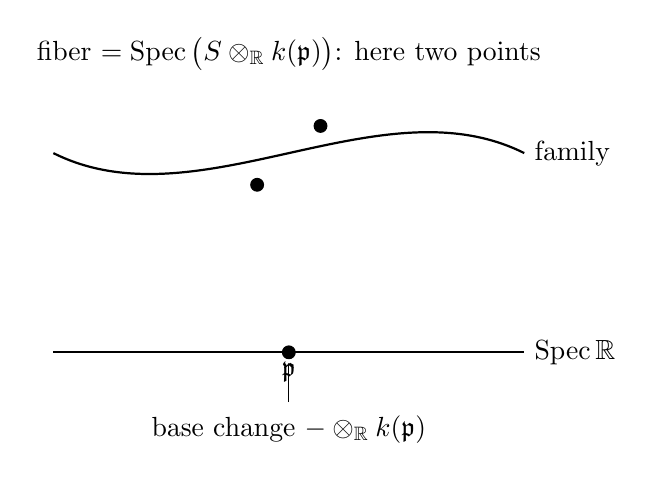
\begin{tikzpicture}[scale=1.15]
  \draw[thick] (-2.6,0) -- (2.6,0) node[right] {$\Spec\R$};
  \filldraw (0,0) circle (2pt) node[below] {$\p$};
  \draw[->] (0,-0.55) -- (0,-0.12);
  \node at (0,-0.85) {base change $-\otimes_\R k(\p)$};
  \draw[thick] (-2.6,2.2) .. controls (-1,1.4) and (1,3) .. (2.6,2.2) node[right] {family};
  \filldraw (-0.35,1.85) circle (2pt); \filldraw (0.35,2.5) circle (2pt);
  \node at (0,3.3) {fiber $=\Spec\big(S\otimes_\R k(\p)\big)$: here two points};
\end{tikzpicture}
\caption{Tensoring with the residue field $k(\p)$ extracts the fiber of a family over the point
$\p$ --- evaluation of a module at a point.}
\end{figure}

% ══════════════════════════════════════════════
\section{Nakayama's Lemma}
% ══════════════════════════════════════════════

\begin{theorem}[Nakayama]\label{thm:nakayama}
Let $(R,\m)$ be local and $M$ a finitely generated $R$-module. If $\m M=M$ then $M=0$.
\end{theorem}
\begin{proof}[Proof (determinant trick)]
Let $M=Rm_1+\cdots+Rm_n$. From $\m M=M$ write $m_i=\sum_j a_{ij}m_j$ with $a_{ij}\in\m$. With
$A=(a_{ij})$ and $I_n$ the identity matrix, $(I_n-A)\cdot(m_1,\dots,m_n)^{\mathsf T}=0$. Multiplying by
the adjugate of $I_n-A$ gives $\det(I_n-A)\,m_i=0$ for all $i$, hence $\det(I_n-A)M=0$. Expanding the
determinant, $\det(I_n-A)=1+u$ with $u\in\m$; in a local ring $1+u$ is a unit (else $1\in\m$).
A unit annihilating $M$ forces $M=0$.
\end{proof}

\begin{corollary}\label{cor:nak-1}
If $N\subseteq M$ with $M=N+\m M$ then $N=M$. (Apply Theorem~\ref{thm:nakayama} to $M/N$.)
\end{corollary}

\begin{corollary}[Generators lift]\label{cor:nak-2}
If $m_1,\dots,m_n\in M$ have images spanning the $R/\m$-vector space $M/\m M$, then $m_1,\dots,m_n$
generate $M$. Consequently the minimal number of generators of $M$ equals $\dim_{R/\m}(M/\m M)$.
\end{corollary}
\begin{proof}
Take $N=Rm_1+\cdots+Rm_n$; then $M=N+\m M$, so Corollary~\ref{cor:nak-1} gives $M=N$. Minimality:
any generating set maps to a spanning set of $M/\m M$, and a basis of $M/\m M$ lifts to a minimal
generating set by the first sentence.
\end{proof}

\begin{remark}[Why Nakayama matters here and later]
$M/\m M$ is the \emph{fiber} of $M$ at the point $\m$ (Figure~1); Nakayama says a f.g.\ module is
controlled by its fiber. This is the engine behind: generators of stalks of sheaves (S26--S28),
tangent spaces and smoothness (S30), and the equivalence ``flat + f.g.\ over local $=$ free''
that makes flatness the algebraic form of ``vector bundles vary continuously'' (S30).
\end{remark}

% ══════════════════════════════════════════════
\section{Flatness}
% ══════════════════════════════════════════════

\begin{definition}[Flat module]
$M$ is \textbf{flat} if $M\otimes_R-$ preserves exactness of every s.e.s.; equivalently, for every
injective $A\hookrightarrow B$, the map $A\otimes M\hookrightarrow B\otimes M$ is injective.
\end{definition}

\begin{example}\label{ex:flat}
\begin{itemize}
  \item Free modules are flat (tensor with $R^n$ is a direct sum of copies).
  \item Direct sums and direct limits of flat modules are flat.
  \item $S^{-1}R$ is flat over $R$: localization is exact (Proposition~\ref{prop:loc-flat}).
  \item $\Z/n$ is \emph{not} flat over $\Z$ (Example~\ref{ex:not-left-exact} with $M=\Z/n$).
  \item Fields are flat; more generally any localization is (previous item).
\end{itemize}
\end{example}

\begin{proposition}[Localization is exact, hence flat]\label{prop:loc-flat}
For a multiplicatively closed $S\subseteq R$, the functor $M\mapsto S^{-1}M$ is exact; in particular
$S^{-1}R$ is a flat $R$-module, and $S^{-1}M\cong S^{-1}R\otimes_R M$.
\end{proposition}
\begin{proof}
The isomorphism $\frac1s\otimes m\leftrightarrow\frac{m}{s}$ is well-defined by the universal property
(Theorem~\ref{thm:tensor-up}). Exactness: surjectivity and $\im\subseteq\ker$ are formal; for
injectivity, if $\frac{a}{s}\in S^{-1}A$ maps to $0$ in $S^{-1}B$ then $t\,f(a)=0$ in $B$ for some
$t\in S$, hence $f(ta)=0$ so $ta\in\ker f=0$, whence $\frac{a}{s}=\frac{ta}{ts}=0$ in $S^{-1}A$.
\end{proof}

\begin{remark}[Preview: flatness in S30 and in homological algebra]
Over a local ring, \emph{flat + finitely presented $=$ free}; globally, flat + f.g.\ $=$
\emph{locally free} (a vector bundle). \'Etale maps (S30) are flat + unramified: geometrically
``local isomorphisms'', algebraically ``fibers are finite sets of reduced points''. Homologically,
flatness is the vanishing of $\Tor$ (S43): $M$ flat $\iff\Tor_1^R(M,N)=0$ for all $N$. Thus this
session's right-exactness is the seed of the entire derived-functor machine of S42--S45.
\end{remark}

% ══════════════════════════════════════════════
\section{Exercises}
% ══════════════════════════════════════════════
\begin{exercise}
Prove $\Z/m\otimes_\Z\Z/n\cong\Z/(m,n)$ directly from the universal property
(Theorem~\ref{thm:tensor-up}), without using right-exactness.
\end{exercise}
\begin{exercise}
Show $\Q/\Z\otimes_\Z\Q=0$. Conclude that $\Q/\Z$ is neither flat nor free over $\Z$.
\end{exercise}
\begin{exercise}
Prove Theorem~\ref{thm:right-exact} in full detail, including the well-definedness of $\beta$.
\end{exercise}
\begin{exercise}
Using Example~\ref{ex:not-left-exact}, exhibit an injective map $A\hookrightarrow B$ such that
$A\otimes\Z/2\to B\otimes\Z/2$ is \emph{not} injective.
\end{exercise}
\begin{exercise}
Prove the splitting lemma (Proposition~\ref{prop:split}) in all directions, and give a s.e.s.\ of
$\Z$-modules that does \emph{not} split.
\end{exercise}
\begin{exercise}
Reprove Nakayama (Theorem~\ref{thm:nakayama}) for $n=1$ and $n=2$ generators by hand, then deduce
Corollaries~\ref{cor:nak-1} and~\ref{cor:nak-2} from the general case.
\end{exercise}
\begin{exercise}
Let $(R,\m)$ be local and $M$ f.g.\ with $M/\m M=0$. Show $M=0$. Give an example of a
\emph{non}-f.g.\ module over a local ring with $M=\m M\neq0$ (hint: $M=R/\m$-vector spaces of
infinite dimension won't work; try $M=\Q$ over $\Z_{(p)}$... check carefully).
\end{exercise}
\begin{exercise}
Prove $M\otimes_R R/I\cong M/IM$ for any ideal $I$, and interpret it as ``restriction of the family
to the closed subset $V(I)$''.
\end{exercise}
\begin{exercise}
Show $\C\otimes_\R\C\cong\C\oplus\C$ explicitly (idempotents $e_\pm=\frac12(1\otimes1\mp i\otimes i)$),
and identify the two points of $\Spec(\C\otimes_\R\C)$.
\end{exercise}
\begin{exercise}
Prove that $S^{-1}R$ flat over $R$ implies: if $M\hookrightarrow N$ is injective then
$S^{-1}M\hookrightarrow S^{-1}N$ is injective. Conversely, show $\Z_{(p)}$ is flat over $\Z$ but
$\Z/p$ is not.
\end{exercise}
\begin{exercise}
Let $M,N$ be f.g.\ modules over a local ring $(R,\m)$. If $M\otimes_R N=0$, prove $M=0$ or $N=0$
(hint: look at fibers $M/\m M$, $N/\m N$ and use Nakayama).
\end{exercise}
\begin{exercise}
Show that the rank of a free module over a commutative ring is well defined (Proposition in \S1),
and deduce that $R^m\cong R^n\Rightarrow m=n$ even when $R$ has zero-divisors.
\end{exercise}

% ══════════════════════════════════════════════
\section*{Where This Session Feeds the Course}
\addcontentsline{toc}{section}{Where This Session Feeds the Course}
% ══════════════════════════════════════════════
\begin{itemize}
  \item \textbf{Depends on:} S1 (rings, ideals, localization, Krull for maximal ideals).
  \item \textbf{Feeds:} S24 (fractional ideals as modules); S26--S28 (sheaves of modules, stalks,
    fibers $M\otimes k(\p)$); S30 (flat/\'etale/smooth, Jacobian criterion); S32 (K\"ahler differentials);
    S42--S45 (Tor, Ext, cohomology: the derived repair of right-exactness).
  \item \textbf{Unifying thread:} a module is a family of vector spaces over the points of $\Spec R$;
    tensoring with $k(\p)$ evaluates the family at $\p$; base change $S\otimes_R-$ pulls the family
    back along $\Spec S\to\Spec R$; flatness says the fibers vary without jumps.
\end{itemize}

\subsection*{References for this session}
\begin{enumerate}[label={[\arabic*]}]
  \item Atiyah, M.F. \& Macdonald, I.G. \emph{Introduction to Commutative Algebra}, ch.2--3.
  \item Eisenbud, D. \emph{Commutative Algebra with a View Toward Algebraic Geometry}, ch.1, 6--7.
  \item Lang, S. \emph{Algebra}, ch.XVI.
  \item Matsumura, H. \emph{Commutative Ring Theory}, ch.2--3 (Nakayama, flatness).
\end{enumerate}

\vspace{1.5em}
\begin{center}
\rule{0.6\textwidth}{0.4pt}\\[0.5em]
\textit{End of Session S2 --- next: Session S3, Fields, Extensions, and Algebraic Closure}
\end{center}

\end{document}